
%\documentclass[journal=no,submission,spthm]{iacrtrans} 
%\documentclass[twoside]{IEEEtran}
\documentclass{llncs}

\usepackage{listings}
\usepackage{color}

\definecolor{dkgreen}{rgb}{0,0.6,0}
\definecolor{gray}{rgb}{0.5,0.5,0.5}
\definecolor{mauve}{rgb}{0.58,0,0.82}

\lstset{frame=tb,
  language=Java,
  aboveskip=3mm,
  belowskip=3mm,
  showstringspaces=false,
  columns=flexible,
  basicstyle={\small\ttfamily},
  numbers=none,
  numberstyle=\tiny\color{gray},
  keywordstyle=\color{blue},
  commentstyle=\color{dkgreen},
  stringstyle=\color{mauve},
  breaklines=true,
  breakatwhitespace=true,
  tabsize=3
}

\usepackage{algorithm}
\usepackage[]{algorithmic}
\usepackage{pgfplots}
\pgfplotsset{compat=1.16}
\usepackage{graphicx}
\usepackage[english]{babel}
\usepackage[utf8x]{inputenc}
\usepackage[T1]{fontenc}
\usepackage{upgreek}
\makeatletter
\newcommand{\ssymbol}[1]{^{\@fnsymbol{#1}}}
\makeatother
\newcommand{\todo}[0]{\textcolor{yellow}{TODO}}
\usepackage[weather]{ifsym}
\usepackage{xcolor,colortbl}
\usepackage{url}
\usepackage{array}
\usepackage{amsfonts}
\usepackage{amssymb}
\usepackage{amsmath}
\usepackage{graphicx}
\usepackage{mdframed}
\usepackage[colorlinks=false, allcolors=blue]{hyperref}
\usepackage[pdf]{graphviz}
\usepackage{subcaption}
\usepackage{cleveref}

\DeclareMathOperator{\numUses}{numUses}
\DeclareMathOperator{\Tab}{Tab}
\DeclareMathOperator{\CB}{CB}
\DeclareMathOperator{\expiry}{expiry}
\DeclareMathOperator{\Encrypt}{Encrypt}
\DeclareMathOperator{\extra}{extra}
\DeclareMathOperator{\rand}{rand}
\DeclareMathOperator{\oldkey}{old\_key}
\DeclareMathOperator{\newkey}{new\_key}
\DeclareMathOperator{\sk}{sk}
\DeclareMathOperator{\SHA}{SHA}
\DeclareMathOperator{\tok}{tok}

\pgfplotsset{select coords between index/.style 2 args={
    x filter/.code={
        \ifnum\coordindex<#1\def\pgfmathresult{}\fi
        \ifnum\coordindex>#2\def\pgfmathresult{}\fi
    }
}}

\newcounter{algoc}
\setcounter{algoc}{0}
\newtheorem{algo}[algoc]{Algorithm}

\newcounter{prob}
\setcounter{prob}{0}
\newtheorem{Problem}[prob]{Problem}

\newcommand{\ph}[1]{\emph{\bf \color{red}\,[Paul: #1]\,}}
\newcommand{\ab}[1]{\emph{\bf \color{blue}~[Agathe: #1]}}
\newcommand{\cn}[1]{\emph{\bf \color{purple}~[Cyrius: #1]}}
\newcommand{\br}[1]{\emph{\bf \color{green}~[Brice: #1]}}
\newcommand{\di}[1]{\emph{\bf \color{orange}~[Diane: #1]}}
%\usepackage{syntonly}
%\syntaxonly

\begin{document}
\pagestyle{plain}
\title{An upcycling tokenization method for credit card numbers}
\author{The dream team}
\institute{REDOCS 2020%\footnote{ \section*{Acknowledgments}
% This work has been accomplished during the french working session REDOCS’20. REDOCS stands for \textit{Rencontre Entreprises DOCtorants en Sécurité}. It is a one week event, where cybersecurity PhD students are working in groups to solve real life problems proposed by industrial companies. The authors of this work would like to thank the GDR Security for organizing the event. Special thanks go to Pascal Lafourcade and Olivier Blazy who guided them during the whole week. The authors also thank Be-Ys for having proposed this project. They particularly thank Marius Lombard-Platet for having supervised this work.}
}
\maketitle


\begin{abstract}
Internet users are increasingly concerned about their privacy and are looking for ways to protect their data. On top of that, they may rightly fear that companies extract information about them from their online behavior. The process called tokenization allows for the use of identities managed by a trusted third party from which no personal data about the user can be inferred.
We study in this paper tokenization systems allowing one to hide the credit card number of a customer on a webshop. We present here a method for generating and managing tokens using a database. We refer to our approach as \lq\textit{upcycling}\rq~as it allows for regenerating used tokens by maintaining a table of currently valid tokens.
We compare our approach to existing one and analyze the security of our tokenization system. We prove that it satisfies the common specifications for the domain. Finally, we provide measurements from an implementation, that confirms the validity of our approach.\br{Mettre un score}
\end{abstract}


\section{Introduction}
Even under a pseudonym, Internet users leave digital fingerprints behind them. All this data can be studied in order to infer information about the user and their behavior. This is notably done on the largest e-commerce platforms and social networks. In addition, the secure storing not possible for online payment, and there is always risk of data leak. Last years have witnessed numerous episodes of credit cards thefts online, as the Davinci breach~\cite{Krebs2019} in February 2019 (2.15 million stolen credit cards), the Bigbadaboom-II~\cite{Thales2018} in August 2019 (5.13 million stolen credit cards from Hy-Vee users), and the Bigbadaboom-III~\cite{Secureworld2020} in January 2020 (30 million stolen credit cards), to name a few.

In order to reduce this traceability, limit the possible inferences of the data and limit the risk of data leakage, a common approach is to give a temporary identity to the user. This temporary identity, called a token, is delivered by a trusted third-party, called a Token Service Provider (TSP), that serves as a proxy masking the user's real identity.

According to the Census Bureau of the Department of Commerce~\cite{census2020}, the estimate of U.S. retail e-commerce sales for the second quarter of 2020 was \$211.5 billion, an increase of 31.8 percent (±1.2\% of confidence interval) from the first quarter of 2020. In total, the estimated e-commerce sales represent 17\% of total sales. According to other sources, in 2019 there were 2.8 billion credit cards in worldwide~\cite{spend2020}, and the number of credit card transactions in 2017 was estimated to 41 billion credit card transactions in the US~\cite{credit2020}. Therefore, the ability to reuse credit card values over time, e.g., to reallocate expired credit card numbers to another customer is a crucial aspect to take into account in our system assigning temporary credit card numbers to customers.

\subsubsection{Tokenization}
Nowadays, to increase the security of online payments, many payment systems use  ``tokenization''. This process replaces an existing payment card number with a substitute value (the token). This token is then used during a payment transaction, allowing to proceed with the payment without exposing actual bank details. The Token Service Provider associates the original card number with the payment tokens and stores all sensible data securely.

More precisely, the TSP manages the entire life-cycle of tokens. The typical scenario in this context is depicted in Figure~\ref{fig:tokenization-system}:
\begin{enumerate}
    \item \textit{Token Request}: The customer requests a token to the TSP.
    \item \textit{Query}: The TSP queries all data needed for the creation of the token (usually from the card issuer).
    \item \textit{Tokenization}: the TSP creates a token from the Credit Card Number and sends it to the customer.
    \item \textit{Purchase}: The customer purchases an item or service form an online shop and transmits the token number instead of its Credit Card Number
    \item \textit{Payment Request}: The merchant site returns the token to the TSP and claims the payment.
    \item \textit{Detokenization}: The TSP converts the token back to the correct Credit Card Number and transmits the payment request to the card issuer
    \item \textit{Payment}: The card issuer satisfies the payment request from the merchant site.
\end{enumerate}

\begin{figure}
    \centering
    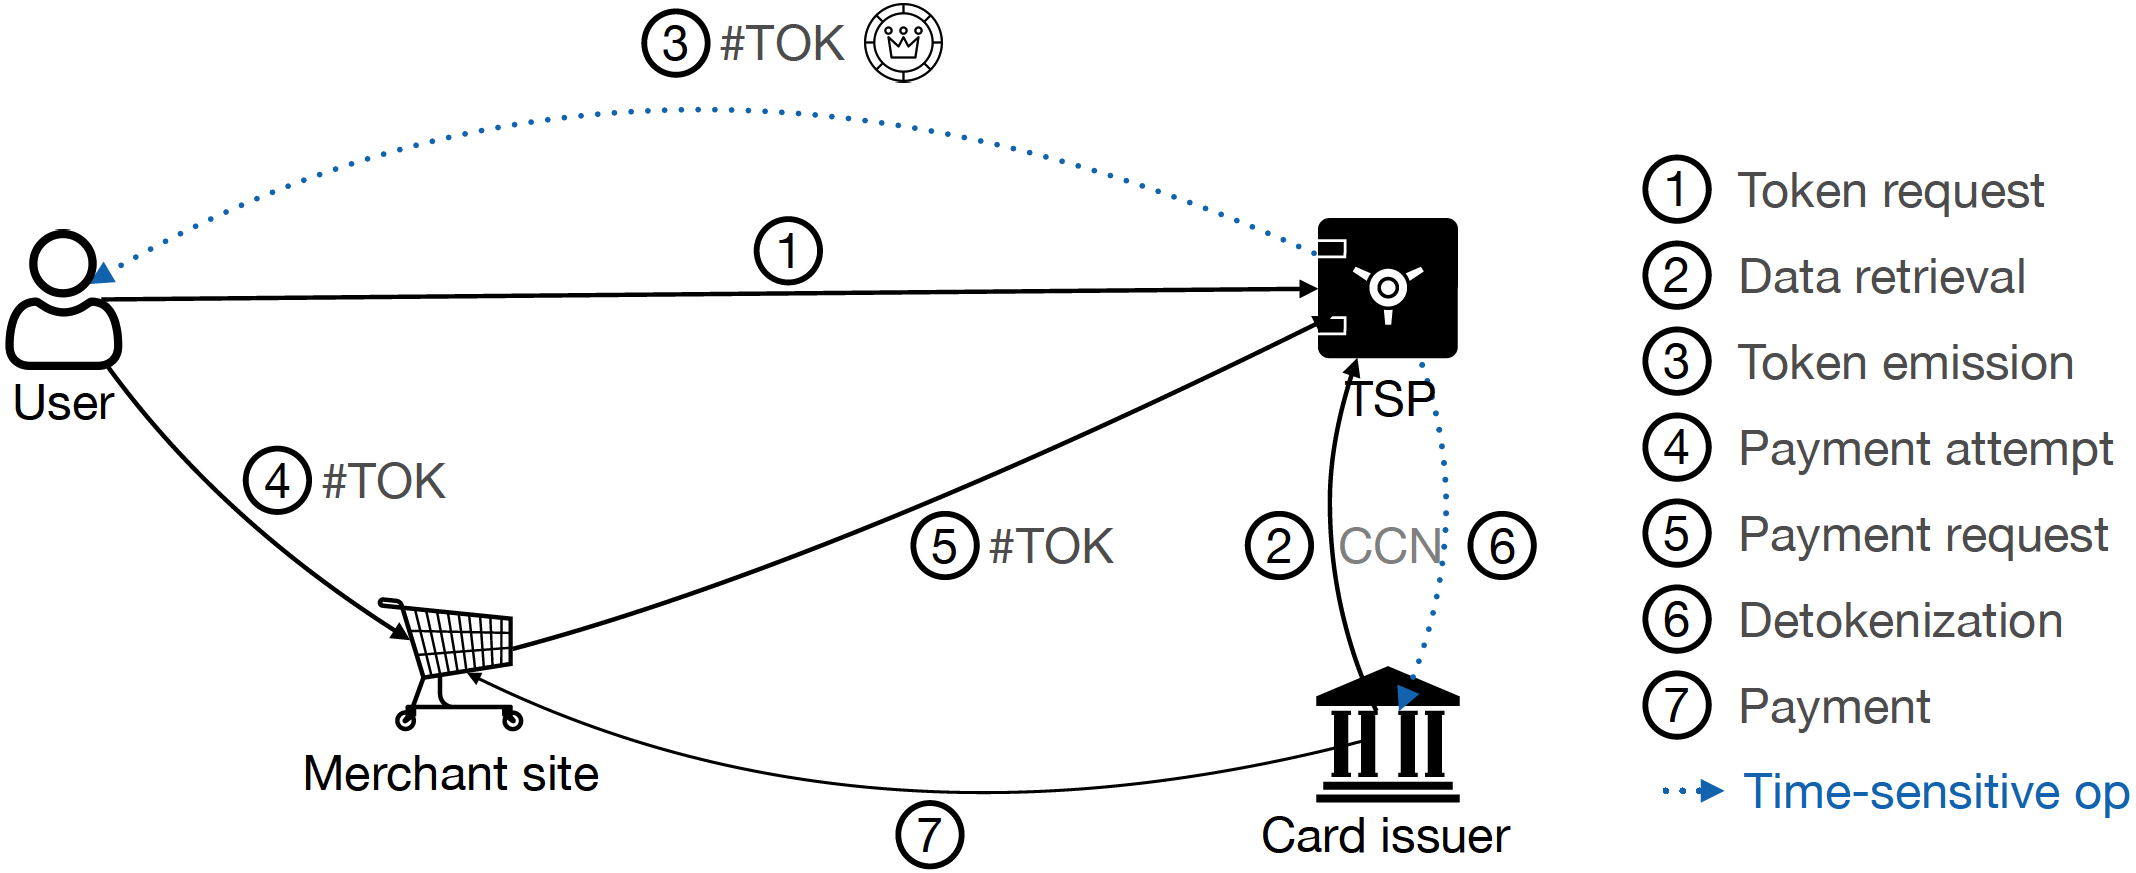
\includegraphics[width=\textwidth]{figures/use_case.png}
    \caption{Tokenization system in our use case}
    \label{fig:tokenization-system}
\end{figure}

The main role of the TSP is the role of token vault: establishing a correspondence between the token and the Credit card number. The TSP can endorse additional responsibilities like domain management (give additional security by limiting the tokens to specific channels or retail domains) and authentication (ensuring the detokenization that the token has been legitimately used by the correct client). In addition, it verifies the identity of the user, asking the user to claim his identity with a password, through multi-authentication, or with its signature, e.g., generated via RSA.

Card issuers can endorse the role of TSP, allowing full control of the tokenization process. Otherwise, card issuers may use a third-party TSP and integrate it with their payment systems.

\subsubsection{CCNs}
Credit card numbers (\textsc{ccn}s) are the identifiers that can be found on any payment cards. These numbers, called primary account numbers (or \textsc{pan}s) consist of a maximum of 19 digits that identify the card issuer and the card holder. They are composed up of three main elements, in accordance with ISO/IEC 7812-1~\cite{ISO78121}:
\begin{enumerate}
    \item The issuer identification number (\textsc{inn}), which corresponds to the leading 8 numerical digits. 
    \item The individual account number, which can be of variable length -- between 1 and 10 digits.
    \item A check digit computed from all the preceding digits of the \textsc{pan} using the Luhn algorithm, also known as the \lq\textit{modulus 10}\rq~algorithm~\cite{Luhn1960}.
\end{enumerate}

The individual account number is usually seven digits long, which amounts to a total of 16 digits in for the \textsc{pan}.

As for the payment token, it is possible to adopt a structure that slightly deviates from the conventional format~\cite{PCI-Guidelines}. For instance, the first four digits can be used to identify the card issuer; the last four digits are fixed and can be used for integrity or error detection purposes in the token (such as a checksum); the remaining 8 digits in the middle identify the token. In the remaining sections of the paper, this format will be considered.

\cn{bien differencier les open digits du whole token}
%\textsc{ccn}s can be stored on 64 bits to include the 16 \textsc{ccn}s digits plus the three \textsc{CVC} digits.

\subsubsection{Specifications}
The specifications for the tokenization systems are listed hereafter.
\begin{enumerate}
    \item \label{item-spec-disting} \textit{Unicity}: Each token should be attributed to at most one user at any given time.
    \item \textit{Expiry time}: A token has a maximal number of uses and/or an expiry date.
    \item \label{item-spec-format-ccn} \textit{Formatting}: The format of the token should be identical to \textsc{ccn}s 
    \item \textit{Distribution}: The distribution of the tokens should match the one of \textsc{ccn}s. \cn{reformuler}
    \item \label{item-spec-linkable} \textit{Unlinkability}: Tokens should not be linkable to one another, or to a user.
    \item \label{item-spec-time} \textit{Timeframe}: Tokenization and Detokenization computation times should not exceed a given timeframe value denoted $Tf$. In this paper, we consider $Tf$ to be 100 ms. \cn{justifier ?}
    \item \label{item-spec-unforgeability}\textit{Unforgeability}: An adversary should be unable to forge an invalid token.
    \item \label{item-sper-reusablilty}\textit{Reusability}: The space of all tokens being smaller than the expected number of token requests, tokens should be able to be issued several times.
    \item \textit{Auditability}: \di{demander à Marius}
    \item \textit{Security}: Any database used should be as secure as possible as long as all previous specifications are validated.
    \item \textit{Dynamic size}: Any database used should be as small as possible as long as all previous specifications are validated. \cn{p-e n'écrire celle ci que si on fait scalable bloom ? }
\end{enumerate}



\subsubsection{Our contributions}
In this paper, we study \textsc{ccn}s tokenization systems. We take a look at existing approaches to create a tokenization system complying with the specifications and then propose our own. We refer to our approach as ``\textit{upcycling}'' as it allows for regenerating used tokens by maintaining a table of currently valid tokens. We propose a proof of concept implementation and study its memory and time performances. Additionally, we study the possibility of adding a database for compliance with extra audit requirements. 

\smallskip

\subsubsection{Organization of the paper}
Section~\ref{sect:background} contains related works on the subject of tokenization systems for \textsc{ccn}s. %contains the study of possible solutions for tokenization systems, knowingly the use of Format Preserving Encryption and the use of a blockchain.
Section~\ref{sect:method} presents our approach and the different algorithms. We study the compliance to the specifications and the impact of different parameters on our system.
Section~\ref{sect:eval} gives experimentation and benchmark results of our proof-of-concept implementation. The source code used for the detection and evaluation is available in the Appendix.\ph{On met le code en Annexe ou on met juste un lien vers le git ? Et dans ce cas là, on met une petite phrase en mode 
"The source code is available as supplementary material and will be made public after acceptance." ou on se fiche de l'anonymat pour les reviews ?}
Section~\ref{sect:conclu} draws conclusions from our work.

\section{Background and related work}\label{sect:background}

In this section, we present the related work on static pre-computed tables, format-preserving encryption (FPE), and space-efficient data structures. We then position our contribution with respect to the described related work. Note that we also considered of a blockchain to proceed to tokenization and detokenization in a secure way with no central authority, and present it in the appendix.

The authors in \cite{Diaz2014} formally define tokenization systems and identify three different systems that solve the problem of tokenization both securely and efficiently: the first one uses format-preserving encryption (FPE) while the two second ones avoid its use. The two latter systems use off-the-shelf cryptographic primitives using ordinary block ciphers, stream ciphers supporting initialization vectors, and physical random number generators. The difference between both relies on whether pairs of token and PAN are stored in the card-vault in the encrypted form or not. The authors also give several security notions and provably secure constructions. However, they do not consider adaptive corruptions and unlike \cite{Cachin2017}, they do not address updatable tokens.
The authors also refer to the Voltage Security solution \cite{Voltage} as the only solution at this time to the tokenization problem with known cryptographic guarantees, using static pre-computed tables.

As a matter of fact, most existing solutions are static and do not provide key updatability, i.e., they do not regularly update the cryptographic keys, while maintaining the tokens' consistency. Therefore in most practical deployments, cryptographic keys must be re-keyed periodically to ensure continued security.
\cite{Cachin2017} constructs two tokenization models for updatable tokenization with key evolution, in which a key exposure does not disclose relations among tokenized data in the past, and where the updates to the tokenized data set can be made by an untrusted entity and preserve the consistency of the data. The authors formally define the security requirements that guarantee unlinkability among different tokens generated from a same user.

\subsection{Format-preserving Encryption}

One common option for the generation of tokens is the use of Format-preserving Encryption (FPE) \cite{Bellare2009}. For simple formats such as the 8 free digits of tokens, FPE can be seen as a key-indexed Pseudorandom Permutations of the set of all values of correct format. The key space can be much greater than the space of correct values, which is also called \textit{domain}.

The FPE has gradually emerged as a useful tool in applied cryptography in recent years. The initial motivation for its use came from the encryption issues commonly raised by companies looking for solutions. For example, a company wants to encrypt distinct and unpredictable 16-digit credit card numbers, but, traditional block cipher will expand data and change format, it requires that we must modify application or database at huge expense \cite{liu2010format}.

The goal of FPE is to avoid the need for a database. The natural use of FPE is to encrypt the individual account digits (and the checksum digit) as the 8 free digits of the token. The validation of the token is then done by decryption of the 8 free digits of the token to retrieve a card number to transmit to the bank for payment. If the token given by the merchant to the TSP is incorrect, the corresponding bank account will be invalid.

For now, the domain size is still big enough to not be in reach of known attacks on \textit{small domains}. For example, in \cite{attacksFPEsmallDomains}, attacks are provided on domains up to 8 bits. Following the attacks discovered in \cite{FPEattacks}, the National Institute of Standards and Technology (NIST) recommends using domains of at least one million elements \cite{NistFPErecommandations}. With one hundred million domains, the \textsc{ccn}s  FPE systems are still out of reach for now, but this should be a concern for a long-lasting system.

The first limitation found in the use of FPE is that the map from users to the 8 open digits is not bijective, since two banks with different fixed digits can issue the same open digits to two different users, e.g., John Doe \texttt{5555 5555 1234 5678} and Michel Dupont \texttt{8888 8888 1234 5678}. Such a scenario would imply that the tokens generated by these users would always be the same. These two users cannot have tokens issued with the same key. Another possibility is to have an injective map from card issuers to Token Service Provider that would avoid this type of conflict e.g. having a single TSP per card issuer.

Supposing that the indexing secret keys are changed regularly, cases would happen where two different card numbers with two different keys yield the same token. In this case, in the verification phase, it would be impossible to differentiate the two tokens (see Specification~\ref{item-spec-disting}) except with the inclusion of additional identification information that would need to be stored. Additionally, the pairs (token, secret key) would anyway be kept in a database in order to know the key that deciphers a given token. Storing these pairs and identification data defeats the advantage of using FPE instead of having a static pre-computed table (knowingly reducing storage space).

On the other hand, if we keep the same secret key across time, it opens the possibility for attackers to trace a token number, since it is permanently linked to the card number. This would not comply with Specification~\ref{item-spec-linkable}.

To summarize, the use of FPE would either create collisions or require a database. In the latter case, it just creates an overhead that can be avoided with a classical table/database.



\subsection{Static pre-computed tables}

We call \textit{static pre-computed tables} those ones containing all possible token values computed by advance. Voltage Security proposed a way to generate and use tokens \cite{Voltage} in 2012, according to the Payment Card Industry Data Security Standards (PCI DSS) requirements \cite{PCI-DSS}, which include for example the need to install and maintain a firewall configuration to protect cardholder data, to protect stored cardholder data, to encrypt transmission of cardholder data across open, public networks, etc. Voltage proposes to compute a static table containing all possible tokens. During a token request, a token is randomly associated to the card number. With a good random number generator and a good management of the table where the tokens are stored, this solution is completely in accordance with the PCI DSS and allows a quick tokenization. For a payment request, it simply checks if the token exists in the table and if it is the case it return the associated bank account.

However, Voltage approach leaves some doubts about the security of the table, which is kept in plain text. And more importantly, no mechanism avoids the saturation of the table. This could be a problem if the maximum number of $10^8$ tokens is reached. For certain this technique allows statistically for a quick tokenization but problems arises whenever the number of tokens increases. What Voltage proposes to tackle this issue is to create a new table when the previous one is too full. However this mechanism increases the detokenization times since multiple tables have to be searched to find the correct bank account. Additionally this creates the need for more data storage space.

Although \cite{Cachin2017} provides key updatability, it does not allow for table cleaning and token reusability. Up to our knowledge, we are the first to provide all of these features. Our proposition allows to have a dynamic table which is more portable. Moreover, we propose a method that regularly cleans the table considering the expiry time of tokens and their maximum number of uses. Hence, our system allows to upcycle the token values that are no longer in use in order to ensure the sustainability of our system while using a limited number of tokens.


\section{Our upcycling tokenization method}\label{sect:method}

\cn{TODO}
In this section, we introduce our upcycling tokenization method. In particular, we study the impact of several parameters on our system and give a proof-of-concept implementation as well as benchmark results.

\subsection{System overview}

Our approach is a modification of Voltage's static pre-computed table that will integrate a cleaning mechanism. This way, there is no need to create a new table every time the previous one starts to be too full. Additionally, we encrypt the table for more security, include a mechanism for updating encryption keys, as well as a mechanism to detect unintended modifications in the table.

The basis of our approach is the creation of a table in RAM indexed by the token numbers, which therefore consists of $n_{\max}$ rows. To retrieve data from a token, we thus have to consult row of the table corresponding to the token for which payment is requested. A row is thus composed of:
\begin{itemize}
    \item a card number $\#\CB$, stored on 64 bits to include the 16 \textsc{ccn}s digits plus the three \textsc{CVC} digits.
    % This is necessary for the transaction to proceed, especially during the detokenization step. 
    \item a random number $\rand$ used to generate the token (32 bits). It allows the verification of the row during the \textit{Clean\_table} operation.
    \item a timestamp $\expiry$, which could be expressed in seconds and thus stored over 32 bits, or expressed with a larger range and stored over 64 bits. It indicates the expiry date of the token.
    \item a counter $\numUses$ of the remaining uses of the token. An 8-bit integer is enough for the predicted use of the tokens.
    \item If the tokenization scheme includes an authentication mechanism, all data needed should be stored in the row, e.g., password, verification keys, phone number for multi-factor authentication.
\end{itemize}

The table should be created contiguous in memory so that the access to the $n^\text{th}$ element could be done by calculating the offset from the first element. This way, tokens are perfectly indexed by their value. This allows keeping a constant access time for lookup while keeping a minimal database space (Specification~\ref{item-spec-time}). For security purposes, it is also recommended that the database should be encrypted via a secret key. We assume all randomness generators to be cryptographically strong.

Also note that we considered the use of hash tables instead of an exact table. However, one essential requirement of our algorithm is its scalability, thus we should avoid relying on hash tables whose too high load factor would cause performance degradation. Therefore, we design in our implementation the use of an exact table. The fact we cannot find duplicate values exempts us from the use of a hash table. Unlike using hash tables, the size of our table is strictly equal to the number of keys. In our system, we rely on a function that keeps generating new tokens if one already belongs to the table in order not to handle the storage of duplicate values. Otherwise, we would need to add a parameter to differentiate between two identical token values from two users. For instance, we could use the customer's signature containing its name, identifier, or a personal signature. An alternative version of our algorithm would consist in leveraging hash tables to handle the storage of duplicate values. In addition to hash tables, sketches such as Bloom and Cuckoo filters are both fast and compact space-efficient data structures that produce lower space overhead than hash tables.
% Variants of these filters exist to dynamically adapt the size depending on the number of stored elements, so that the size of the table varies with the number of stored elements. In our current implementation, the default size of the table is the maximum number of elements (i.e., set to $10^8$ in our implementation), no matter the number of elements effectively contained. A variant of bloom filters known as scalable Bloom filters \cite{Almeida2007} is designed to adapt dynamically to the number of stored elements while keeping a minimum false positive probability. In the future, one could imagine that card numbers and tokens would cover $m$ digits, with $m$ greater than 8 as in our current implementation. In this case, adapting the size of the table to the number of stored values would save significant place, compared to allocating space for a table containing $n_{\max} = 10^m$ entries by default, no matter the number of elements effectively stored.

\subsection{Description of the functions}

The three following functions enable one to complete the whole tokenization and detokenization process, as well as the maintenance of the table. %The tokenization (\textit{Token\_request}) and detokenization (\textit{Token\_payment\_request}) operations are performed whenever an customer sends a request to get a token from his card number, while 
The cleaning of the table (\textit{Clean\_table}) is executed to a rate defined by the TSP e.g. once a week or according to the use rate of the system. Hereafter follows a detailed description of each of the processes.

\subsubsection{Tokenization}
The tokenization process consists in generating a token $\tok$ from a card number $\#\CB$. It also implies to store the data concerning the user in order to proceed with subsequent payment requests. The algorithm \textit{Token\_request}$(\Tab, \#\CB , \numUses, \expiry, \extra, \sk)$ takes as input the table $\Tab$, the credit card number of the user $\#\CB$, the maximal number of uses of the token $\numUses$, a timestamp $\expiry$ corresponding to the validity limit of the token, any extra information $\extra$ that would be useful to retrieve at the time of detokenization (e.g. authentication data), and the system's secret key $\sk$. The algorithm picks uniformly a 32 bit $\rand$ and computes the following, given $n_{\max}$ the number of entries by default in the table: 
$$\tok = \SHA_{224}(\rand) \mod n_{\max} $$
\cn{pourquoi faire ça et pas juste rand(10\^8)}
This way, a token is generated by hashing the random number $\rand$ and reducing it to the token space by carrying out a modulo $n_{\max}$ operation on it. Then, it checks whether $\tok$ corresponds to an empty row of the table. If the same token already exists and is valid, then the process restarts with a fresh $\rand$ value until a new token is generated. When the row is empty, it inserts $\textit{Encrypt}_{\sk} (\#\CB | \numUses | \expiry | \rand | \extra)$ in $\Tab$. This $\tok$ is then formatted properly to follow the \textsc{ccn}s format (starting digits and checksums are added). The algorithm outputs the completed token. If no valid token has been found within the given timeframe $Tf$, the process terminates.

%  ajouter dans token\_request signature du client / 
% fonction à part verif_signature, appelée par token\_request, e.g., sur 8 bits --> RSA
Simultaneously, the algorithm \textit{Verify\_signature} is called by \textit{Token\_request} and aims to verify the client's signature stored on 8 bits. The RSA public-key cryptosystem is widely used for secure data transmission. The user must first create and publish a public key based on two large prime numbers, along with an auxiliary value. The prime numbers are kept secret and stored on the client side. When receiving a tokenization request, the bank must first verify the client's authenticity: the client is asked to sign his messages with his prime numbers, then the bank is able to decipher them using the client's public key and check that the signature corresponds to the client. We further detail this method as well as multi-factor authentication in Section \ref{sect:unforgeability}.

\subsubsection{Detokenization}
The detokenization process consists in retrieving a credit card number $\#\CB$ from a token $\tok$. The algorithm \textit{Token\_payment\_request}$(\Tab, \tok, \sk)$ takes as input the table $\Tab$ and the token $\tok$ to verify. It checks whether the table row indexed by $\tok$ is empty or not. If it is empty, the token is invalid and the algorithm stops, otherwise, the row is deciphered to retrieve $(\#\CB | \numUses | \expiry | \rand | \extra)$. If $\expiry$ is lesser than the time of computation, the row is deleted and the algorithm stops. Else, the \textsc{ccn} is then returned to the bank. Additionally, $\numUses$ is decremented, if it reaches 0, the row is deleted. The row is kept encrypted in the database.

\subsubsection{Cleaning the table}
The table has to be cleaned regularly in order to allow the reuse of the token. It is important to allow the reuse of tokens because there are only $n\_{max}$ possible valid tokens that can be used at the same time. To perform a cleaning, each row of the table is checked. The algorithm \textit{Clean\_table}$(\Tab,\sk)$ takes as input the table $\Tab$. For all rows, it deciphers the row to retrieve $(\#\CB | \numUses | \expiry | \rand | \extra)$. The number of remaining uses and the expiry date are verified. If the validity date has passed or if the maximum number of times the token has been used is reached, then the row is erased. This operation should be executed periodically according to the expected quantity of decaying tokens. In addition, if the information needs to be retained for possible auditing, then the information is moved to a database specifically designed to keep track of past tokens and transactions. The algorithm \textit{Clean\_table} checks the following:
\begin{itemize}
    \item Whether $\#\CB$ is a valid \textsc{ccn} by verifying the checksum of the \textsc{ccn}.
    \item Whether $\numUses$ is greater than zero.
    \item Whether $\expiry$ is a date in the future
    \item Whether the $\SHA_{224}(\rand)\bmod n_{\max}$ is the index of the row.
\end{itemize}
In any of these cases, the row is invalid and so is deleted.

Note that for additional security, we can detect modifications in the table to all fields except $\numUses$. For this, Token\_request is modified to hash $(\#\CB | \expiry | \rand | \extra)$. The Clean\_table function checks whether this value is the correct index of the row. If this is not the case, that means that a field changed. Since the value of $\numUses$ changes by design, it cannot be included in this verification process.

Also, keeping the same secret key for a long time can be insecure, notably for social engineering attacks. In order to change regularly the secret key, Clean\_table may also be used as a key updater by taking as inputs $\oldkey$, $\newkey$. Each row is deciphered with $\oldkey$, and after normal operations, the row is inserted enciphered with $\newkey$.

\subsection{Proofs of security}\label{sect:proof}

We prove that given a correct set of parameters, each specification is validated by our approach. Note that in our implementation, we choose $n_{\max}$ equal to $10^8$ corresponding to the 8-digit token numbers and and $Tf = 400,00$ based on results from \texttt{openssl} speed tests.
\begin{enumerate}
    \item \textit{Each token should be attributed to at most one user at any given time.} This is validated by the fact that Token\_request only returns a non-existing token.
    \item \textit{A token has a maximal number of uses and an expiry date.} This is guaranteed by the verification process during Token\_payment\_request and the fact that $\numUses$ is decremented after each use.
    \item \textit{The format of the token should be identical to \textsc{ccn}.} This is done by the formatting step at the end of Token\_request.
    \item \textit{The distribution of the tokens should match the one of \textsc{ccn}.} Any newly issued token has a number taken from a distribution indistinguishable from a uniform distribution. Since the remainder of $2^{224}$ modulo $n_{\max} = 10^8$ is $10,249,216 \approx 2^{23.3}$, the chance of picking an element that would cause a difference from the uniform distribution is $\frac{2^{23.3}}{2^{224}} = \frac{1}{2^{200.7}}$, which implies that there is no distinguisher from the uniform distribution up to a security parameter of 200. \cn{maj pour 2 32}
    \item \textit{Tokens should not be linkable to one another, or to a user.} Because we added random values into the hash, there is no information deductible from multiple tokens.
    \item \textit{Tokenization and Detokenization computation times should not exceed a given timeframe $Tf$ value.} We can guarantee the probability of failure to deliver a new token up to an arbitrary high-security parameter. However, the implementation and the value of $Tf$ have an impact that we quantified in the upcoming paragraph. 
    
    \item \textit{An adversary should be unable to forge an invalid token. } Without modification of the overall tokenization scheme as presented in \cite{ref}, a merchant site could submit a random illegitimate token and request a payment. By doing this, it would have a probability to "land" on an existing token equal to the number of currently valid tokens divided by the total number of tokens. In a token space of $10^8$, this causes a lot of design constraints. However, we propose a modification of the tokenization scheme presented in \cite{otherref}.
    
\end{enumerate}

\subsubsection{Additional proof on the probability of failing to generate a token}

Let us consider a token space of size $n_{\max}$, the number of already generated tokens $n$ and the number of tries $T$ to generate a new token that can be done in the given timeframe $Tf$. We study the maximum $n$, such that the probability of a failure to create a new token is smaller than $2^{-\lambda}$, where $\lambda$ is the security parameter. The probability of failure is the probability of obtaining consecutively $T$ already existing tokens, which happens with a probability of $\frac{n}{n_{\max}}$. Thus we obtain the following inequality:
\begin{equation}\label{eq:fill_rate}
\bigg(\frac{n}{n_{\max}}\bigg)^{T} <\frac{1}{2^\lambda}\iff
n <2^{\log_2(n_{\max})-\frac{\lambda}{T}}.
\end{equation}


\subsubsection{Unforgeability}\label{sect:unforgeability}

We propose hereafter a mechanism to prevent the risk of an attacker that would forge tokens. When the Token Service Provider receives a token from the merchant site, it must first verify the user's identity. One possibility to do so is to ask the merchant site for a signature containing the user's information to verify the user's identity. If this signature is cryptographically secure there is no way to link signatures to one another or to the user issuing them.

Another possibility to reach this property is to rely on multi-factor authentication. Basically, a randomly generated token has $\frac{n}{n_{\max}}$ chances to effectively belong to the table. A good protection mechanism can require an interaction with the user possessing the legitimate token. The bank can verify the identity of the user through multi-factor authentication. A basic implementation would consist in asking the user to manually validate the operation from his/her own device, in order to claim his/her identity and thus validate the transaction.
With this verification, a legitimate user could validate his spending to his bank without transmitting information to the merchant site, while someone that would like to forge tokens would be easily detected.

\subsubsection{Database audit}

In addition to the storage of token values in the table, we consider the use of an external database for permanent data storage. It would allow the sustainability of our system by storing the history of transactions, through not time-sensitive operations. Two types of operations could be performed, as: \textit{1)} logging every operation into the database, and \textit{2)} data cleaning that would be performed, e.g., once a week, to remove the tokens whose validity time is expired and storing them in the database as well.

\section{Evaluation}\label{sect:eval}

We decided to use the C language to have good memory management. Good memory management allows us not only to reduce the amount of RAM used, but also to reduce the token generation time by decreasing the number of bits to be covered. For the sake of reproducibility, our source code is publicly available in the appendix.
% We performed our experiments on a 2017 MacBook Pro with 2.3 GHz Intel Core i5 Processor and 16GB RAM. \ab{Diane: mettre à jour avec les specs du serveur}
\par We performed each experiment on an Intel(R) Xeon(R) CPU E5-2695 v4 @ 2.10GHz CPU. Each processor have an average speed of 2600.198MHz, a   minimal speed of 1200MHz and a maximum speed of 3300MHZ.For each experiment we generated tokens corresponding to credit cards taken randomly and then we filled our table with the corresponding information. We generated tokens up to the first token generated in more than 0.1 second, which is the timeframe we set. In other words, for each experiment, we tokenized until our tokenization was done in more than 0.1 second. We then repeated filling the table in this way 10 times to obtain an average of 10 fills.
\par Our results showed that before a tokenization takes longer than 0.1 seconds, the table can be filled to an average of 99.976\% with a standard derivation of 0.005\%. In other words, we can perform a tokenization with the confidence that the tokenization will take less than 0.1 seconds as long as the table is filled to 99.97\% or less. The average tokenization time observed during table filling until the first failure (tokenization in more than 0.1 second) is 2.56E-05 seconds. In addition, table filling up to the first failure takes an average of 2770 seconds with a standard derivation of 1.9\%.
\par Finally, we also measured the average time to clean the table. This operation consists in going through all the lines of the table and for each line to check that the token corresponds to the registered credit card, that the maximum number of uses has not been reached and that the expiration date has not been exceeded.  If one of these criteria is not checked, then the row is deleted. The average time for cleaning the table is 62.19 seconds with a standard derivation of 1.5\%.

\subsection{RAM usage} 

The theoretical amount of RAM usage depends on the encryption design of the table. Depending on the security requirements, one can decide whether to encrypt the table or not. If it is the case, the table would be encrypted with Advanced Encryption Standard (AES) and 128-bit blocks as it is currently the most secured one and ... \ab{add justif + ref}. Since the data are stored on 162 bits, the encryption would be done on 2 blocks of 128 bits. In addition, as $n_{\max} = 10^8$ rows have to be stored, $25.6$GB of RAM are necessary for the storage of the encrypted table. If we choose not to encrypt the table, only $16.8$ GB of RAM are used for storage.

Since our implementation uses C structures, our table is a table of structures and is therefore stored on SSD memory and not in RAM. Hence, the total amount of RAM usage is equal to $3.2$GB only. Each structure, i.e., each row, uses only 32 bits of RAM, thus it represents $3.2$GB of RAM usage for the $10^8$ rows. However, if the table is encrypted, the structure can not be used efficiently and the data must be stored in RAM. In that case, the theoretical number of RAM usage, i.e, $25.6$GB, is reached.

\subsection{Filling rate}

Given the formula $n <2^{\log_2(n_{\max})-\frac{\lambda}{T}}$ found in Section~\ref{sect:proof}, the theoretical filling rate of the table before a failure occurs with a probability over $2^{-256}$ and 400,000 tries per $Tf$ equals to $99.92\%$. In other words, the probability of failure becomes larger than $2^{-256}$ when the table is more than $99.92\%$ filled. Our experiments show that the average filling rate before a failure occurs is about $99.998\%$. This is due to the fact that even after $99.92\%$ of filling, there is still a high chance that valid tokens are generated.

The timeframe used is $100$ms, that is to say, that a failure occurs when a valid token has not been generated in $100$ms. The number of trials that our implementation gives per timeframe is about $7220$. By using a faster random generator, this number would be higher. The random generator does not have to be a cryptographic generator, but only to guarantee the uniformity of the generated numbers. \textcolor{purple}{contre exemple: un compteur a une distrib uniforme et est attaquable}

As a result, we show that the theoretical filling rate $n$ of the table must be lower than $2^{\log_2(n_{\max})-\frac{\lambda}{T}}$ in order to insert a new token without collision within the given timeframe $Tf$. By using $Tf = 400,000$ and $\lambda=128$, with this formula, one can achieve a theoretical table filling rate equal to 99.92\%, as illustrated in Figure~\ref{fig:3d-plot}. In addition, the Figure shows the table filling rate value obtained through our assessment. For $Tf=7,221$ and $\lambda=256$, the real table filling rate obtained is equal to 97.57\%.

\begin{figure}
    \centering
    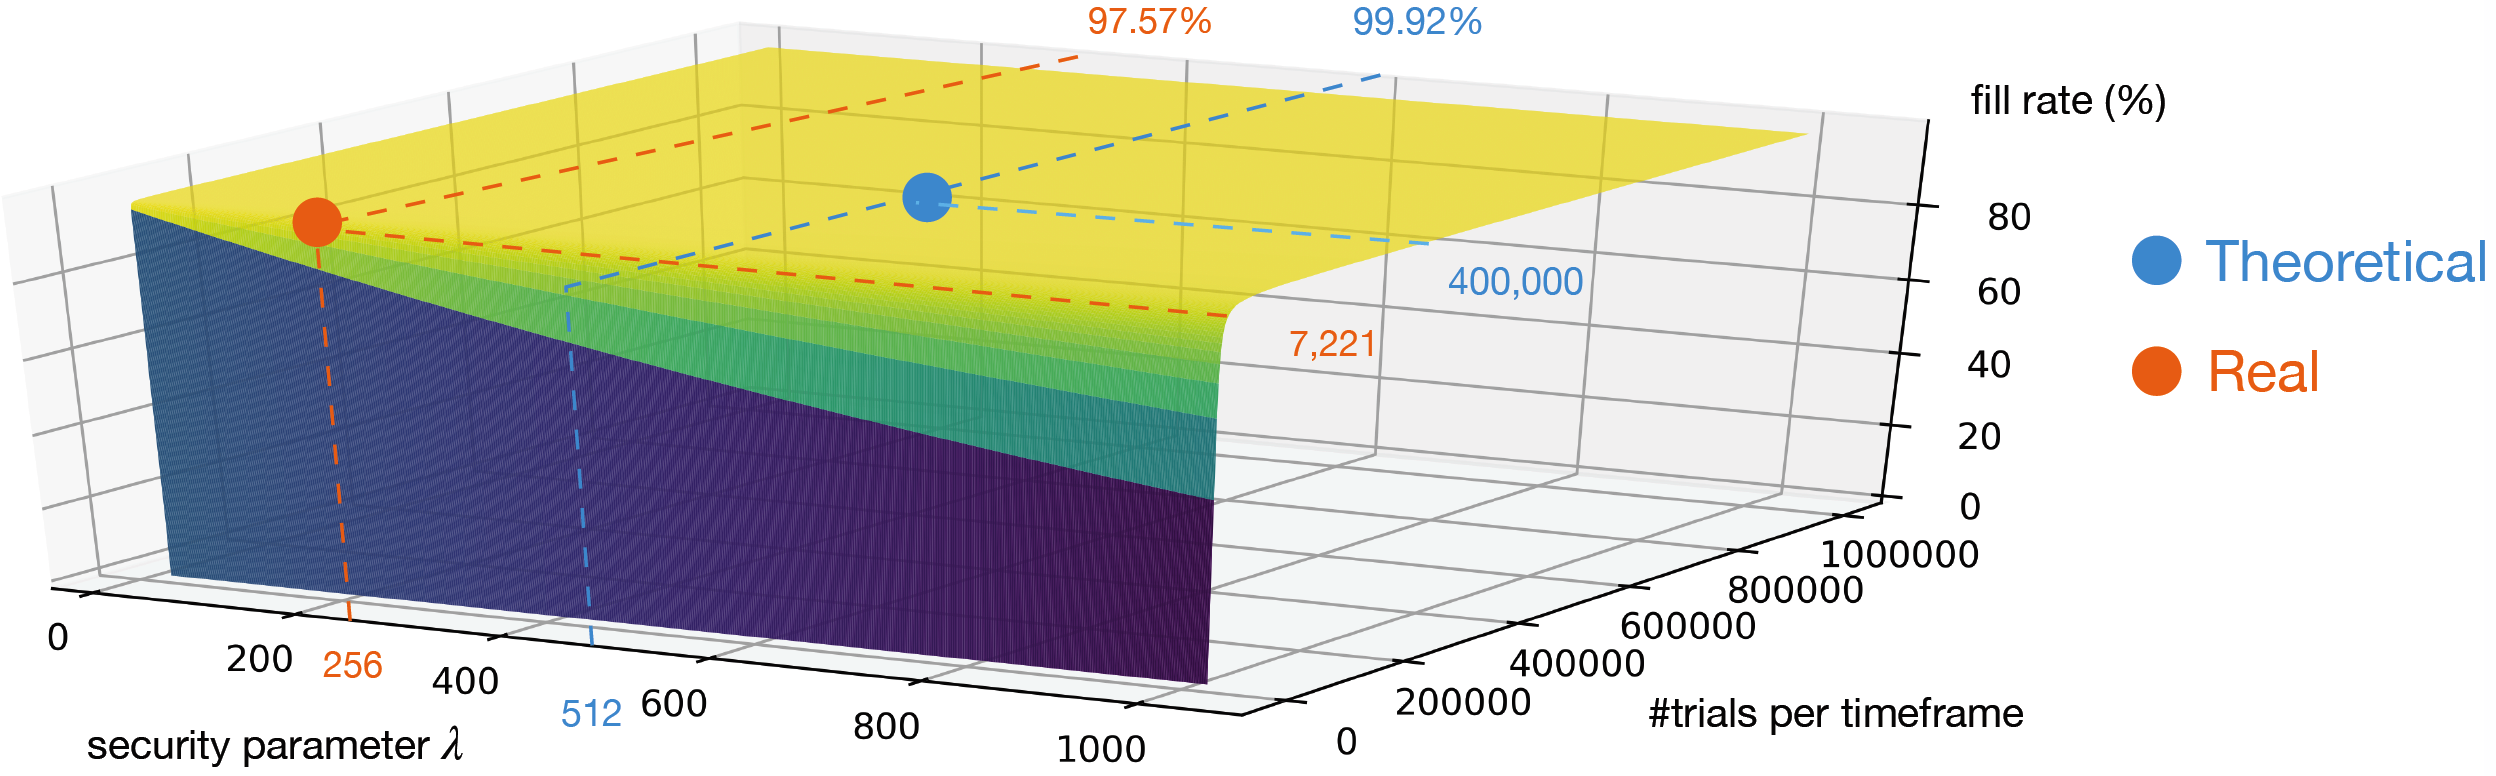
\includegraphics[width=\textwidth]{figures/3d_plot}
    \caption{Theoretical and real table filling rates values, achieved for several combinations of $\lambda$ and $Tf$.}
    \label{fig:3d-plot}
\end{figure}

We now execute the whole tokenization process and we evaluate several metrics: the maximum table filling rate, the index of the first failure, the index of last row, the minimum and maximum number of trials before inserting a correct value, and the time needed to generate the table.
Hereafter, Figure~\ref{fig:boxplot} shows the box plot of these metrics computed for 10 occurrences of this tokenization process. We observe that the median of the maximum table filling rate approximately equals $99.90\%$, which is very high, with a small standard deviation. The median time to generate the table is near 1340 seconds (22 minutes and 40 seconds), also with a small standard deviation.

\begin{figure}
    \centering
    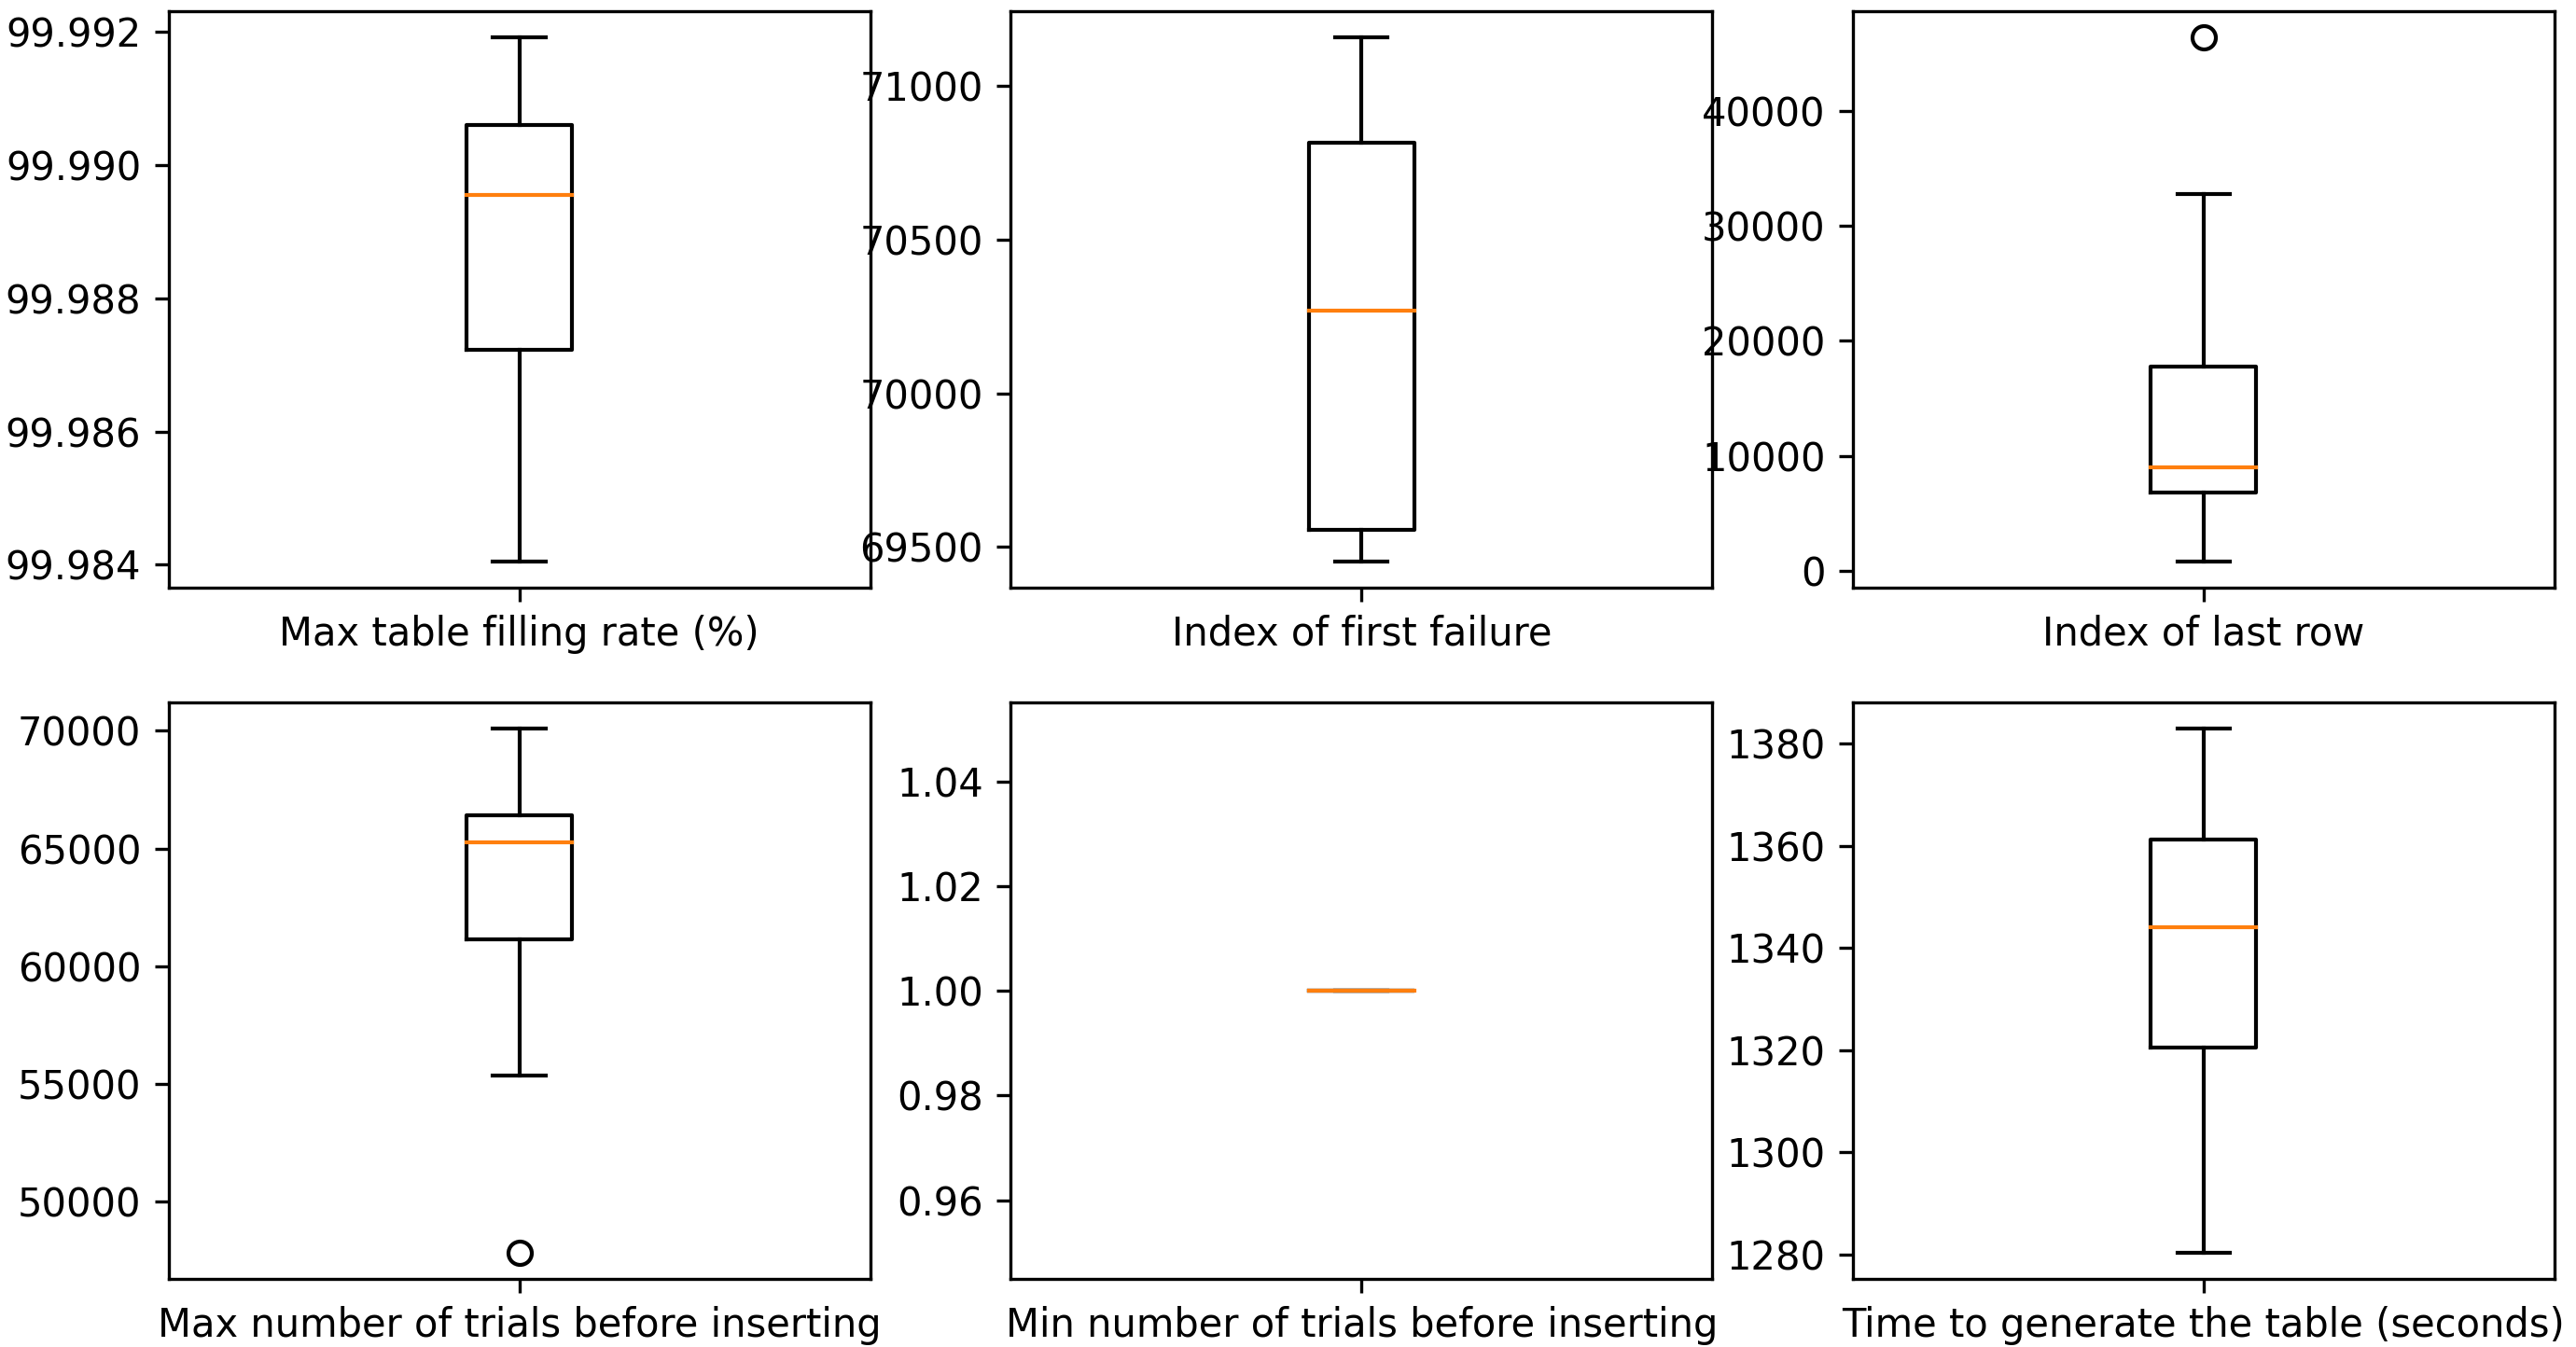
\includegraphics[width=\textwidth]{figures/boxplot}
    \caption{Box plot of values for 10 occurrences of tokenization with tables of $10^8$ rows.}
    \label{fig:boxplot}
\end{figure}

\subsection{Detokenization and cleaning table time}
\br{Fill me, plz! :). This subsection is asking help! :) }

\section{Conclusion}\label{sect:conclu}

\cn{ouverture résilience ? }
\cn{ouverture tabelau d'adresses}
In this paper, we propose a solution for tokenization systems for Credit card numbers. This system is based on the possibility to have the full table of tokens in RAM and so computations are fast enough to guarantee a tokenization without collision. As a result, we found that we can achieve token generation and storage within the given timeframe until the table filling rate reaches to 99.92\% theoretically, and 97.57\% according to our assessment.
We additionally study the inclusion of extra mechanisms to prevent against counterfeited tokens, to allow for a database audit, and to reduce the table size.



\section*{Appendix}\label{appendix:code}

We provide hereafter the source code for tokenization, detokenization, and cleaning of the table, that we used for our evaluation. We also insert a study on whether applying a blockchain to our system would be feasible.

\textbf{Source code}

% insert source code

\textbf{Study on the blockchain applicability}

A possible perspective in order to manage the tokens would be to use a blockchain.
Such a solution would let the users being anonymous with respect to the server, which is an interesting additional property.
Unfortunately, this solution is not feasible in the context of our setting, in particular with the magnitude of $Tf$ (a typical value would be $100$~ms). The security of the blockchain consensus relies on the proof of work that does not fit with this value of timeframe. Different blockchain systems show different speeds for deploying, invoking, and executing smart contracts. In \cite{Ricci2019}, authors introduce a simple queueing theory model to characterize the delay experienced by Bitcoin transactions. They observed that roughly 90\% of all transactions are confirmed within 33 minutes, which would be far too long in our near real-time setting. \cite{Zheng2018} proposes a scalable framework for monitoring the real-time blockchain performances and achieves up to 5.6 Ethereum transactions per second. Broadly speaking, each block of the Bitcoin (respectively Ethereum) blockchain is obtained after a few minutes (respectively a few seconds), but this is still much larger than for conventional credit card systems. Using a blockchain to generate \textsc{ccn}s tokens would generate timeframes of approximately the same magnitude as for Blockchain or Ethereum, i.e., of several seconds or minutes in the worst case, which is far too high compared to our $100$~ms $Tf$ parameter.

\textbf{Space-efficient data structures}
% \cn{passer en annexe en tant que justification du scalable bloom filter si jamais on en implemente un ?}
Different hashing strategies exist to resolve collisions in hash tables:
\begin{itemize}
    \item \textbf{Closed addressing} strategies rely on additional data structures to store all elements with hash collisions, e.g., with linked lists or binary search trees, as separate chaining.
    \item \textbf{Perfect addressing} strategies choose hash functions so that collisions cannot happen, and rehash or move elements when they do. Bloom and Cuckoo filters \cite{Bloom1970} are two space-efficient probabilistic data structures used for approximate set membership. They are designed to check whether an element belongs to a set (here the hash table) or not. They enable: \textit{1)} to know with certainty that an item does not belong to the table (thus there are no false negative matches); and \textit{2)} to assess the probability that an item belongs to the table (thus false positive matches are possible). Therefore, duplicate values can be avoided as one rehashes elements whenever there is a collision. However, the number of false positives increases with the size of the table. Unlike Bloom filters, Cuckoo filters propose the advantage to support item deletions.
    \item \textbf{Open addressing} strategies store duplicate values into the same hash table. Such techniques include linear probing, quadratic probing, and double hashing.
\end{itemize}

A major limitation of hashing tables relies on the impact of the load factor on the performances of the system. The load factor is defined as the proportion of slots in the hash table that are used; in other words, the hash table size should be at least $x$ times greater than the number of keys, with $x$ depending on the hashing strategy. When it increases towards 100\%, the number of probes required to find or insert a given key rises dramatically and then requires the expanding of the table. Once the table becomes full, open addressing algorithms may even fail to terminate. The load factor is traditionally capped at 80\% (for which the hash table size would be equal to 1.25 times the number of keys), but often set to 50\% for open addressing strategies, and up to 100\% for separate chaining.
For the cuckoo filter, there is no condition on the table size, but rather on the maximum number of displacements (estimated to 500 operations in \cite{Fan2014}), after which the procedure of recursively finding a vacant bucket becomes unproductive. Several Bloom filter variants exist to address the deletion of items that is not possible by default. However, this incurs a rising in space to retain the same false positive rate as a space-optimized Bloom Filter. Counting Bloom filters \cite{Tarkoma2012} are 3 to 4 times larger, while $d$-left counting Bloom filters \cite{Bonomi2006} use 1.5 times space.

One essential requirement of our algorithm is its scalability, thus we should avoid relying on hash tables whose too high load factor would cause performance degradation. Therefore, we design in our implementation the use of an exact table. The fact we cannot find duplicate values exempts us from the use of a hash table. Unlike using hash tables, the size of our table is strictly equal to the number of keys. In our system, we rely on a function that keeps generating new tokens if one already belongs to the table in order not to handle the storage of duplicate values. Otherwise, we would need to add a parameter to differentiate between two identical token values from two users. For instance, we could use the customer's signature containing its name, identifier, or a personal signature. An alternative version of our algorithm would consist in leveraging hash tables to handle the storage of duplicate values. In addition to hash tables, sketches such as Bloom and Cuckoo filters are both fast and compact space-efficient data structures that produce lower space overhead than hash tables.
Variants of these filters exist to dynamically adapt the size depending on the number of stored elements, so that the size of the table varies with the number of stored elements. In our current implementation, the default size of the table is the maximum number of elements (i.e., set to $10^8$ in our implementation), no matter the number of elements effectively contained. A variant of bloom filters known as scalable Bloom filters \cite{Almeida2007} is designed to adapt dynamically to the number of stored elements while keeping a minimum false positive probability. In the future, one could imagine that card numbers and tokens would cover $m$ digits, with $m$ greater than 8 as in our current implementation. In this case, adapting the size of the table to the number of stored values would save significant place, compared to allocating space for a table containing $n_{\max} = 10^m$ entries by default, no matter the number of elements effectively stored.

\bibliographystyle{IEEEtran}
\bibliography{bibliography}

\end{document}
